
A discrete abstraction over a continuous space uses relations to
describe the behavior of the system over time. Such relations abstract
the underlying relation between concrete states, and concrete paths
can no longer be constructed directly. Instead, search procedueres
like Counter-Example Guided Refinement must be used to find concrete
paths. In general, such search techniques are exponential with respect to
computational resources and memory. As an alternative, we introduce
data driven `enrichment' of abstractions to approximate the concrete
relations underlying the abstract relations. Informally, we use linear
regression to compute affine maps associated with the relations
between two abstract states. We then show how associating the computed
maps with the relations transforms a discrete abstraction into a PWA
transition system.

\subsection{Graph Abstraction}

% The abstraction of the hybrid dynamical system is a a
% paritioning of the combined state-input space $\HybridStates \times
% \Inputs$ into hyper-rectangles or cells $C_i \in \Cells$. The cells are
% pairwise disjoint $C_i \cap C_j \neq \emptyset$ iff $i \neq j$ and
% their union $\bigcup_{C_i\in\Cells}C_i$ is the state-input
% space $\HybridStates \times \Inputs$. The paritions over
% the continuous input-state space are implicitly defined using a quantization
% function $Q_\epsilon$ parameterized by the precision $\epsilon$.
% This further defines an equivalence relations such that
% \[
%     (\vx_i, \vu_i) \equiv (\vx_j, \vu_j) \;\text{iff}\; Q_\epsilon(\vx_i,
%     \vu_i) = Q_\epsilon(\vx_j, \vu_j)
% \]
% In other words, $(\vx_i, \vu_i) \in C_i \; \text{iff} \; C_i =
% Q_\epsilon(\vx_i, \vu_i)$.

% \begin{definition}[Graph Abstraction]
%     The quantization function $Q_\epsilon$ induces a DAG on the discrete
%     abstraction given by a graph $G(V, E)$, where each vertex
%     corresponds to a cell $V_i = C$, and an edge exists between two
%     cells $(C, C') \in E_i$ iff there exist state-input pairs
%     $(\vx,\vu) \in C$, $(\vx', \vu) \in C'$ such that $\vx' =
%     \simulate(\vx, \vu )$.
% \end{definition}

The abstraction of the hybrid dynamical system is a a
paritioning of the hybrid state space $\HybridStates$ into hyper-rectangles or cells $C_i \in \Cells$. The cells are
pairwise disjoint $C_i \cap C_j \neq \emptyset$ iff $i \neq j$ and
their union $\bigcup_{C_i\in\Cells}C_i$ is the state space $\HybridStates$. The paritions over
the continuous state space are implicitly defined using a quantization
function $Q_\epsilon$ parameterized by the precision $\epsilon$.
This further defines an equivalence relations such that $(\vx_i)
\equiv (\vx_j) \;\text{iff}\; Q_\epsilon(\vx_i) = Q_\epsilon(\vx_j)$.
In other words, $(\vx_i) \in C_i \; \text{iff} \; C_i = Q_\epsilon(\vx_i)$.

\begin{definition}[Graph Abstraction]
    The quantization function $Q_\epsilon$ induces a directed acyclic
    graph (DAG) on the discrete
    abstraction given by a graph $G(V, E)$, where each vertex
    corresponds to a cell $V_i = C$, and an edge exists between two
    cells $(C, C') \in E_i$ iff there exist state-input pairs
    $(\vx) \in C$, $(\vx') \in C'$ such that $\vx' =
    \simulate(\vx)$.
\end{definition}



Given a numerical simulator $\simulate$ and an initial abstraction
defined by a quantization function $\quant_\epsilon$ and a time step
$\Delta$, we pick samples and simulate them to explore the abstraction
on the fly to obtain a graph $G$, which has a finite number of
abstract states $C$ (or cells) and edges $(C,C')$ iff $C
\areach{\Delta} C'$.


% \begin{definition}[Abstract State Graph]. Let ∆ > 0 be a fixed time
%     step. The abstract state graph H(∆) for time step ∆ is defined by
%     the set of vertices C, and edges (Ci, Cj ) whenever Ci ∆ Cj . Let
%     C0 denote the collection of initial cells in C, i.e., cells Ci
%     such that Ci ∩ X0 6= ∅. Further, let Cu denote the set of unsafe
%     cells, or cells Cj such that there is a state xj ∈ Cj that reaches
%     an unsafe state y ∈ Xf within time 0 ≤ tj < ∆. The abstraction
% H(∆) is given by D C, ∆ , C0, Cu E .  \end{definition}

Instead of using a CEGAR like loop (used in~\cite{zutshi2014multiple}),
we use the generated trajectories to learn quantitative models
describing the local behavior of the system. These models are defined
by a set of relations $R \subseteq \HybridStates \times \HybridStates$
for each edge of the reachability graph.


\subsection{Enriched Abstraction}


\begin{figure}[!htbp]
\begin{center}
\tikzstyle{line} = [thick]
\tikzstyle{arw} = [->, thick,>=stealth,shorten <=2pt, shorten >=2pt]
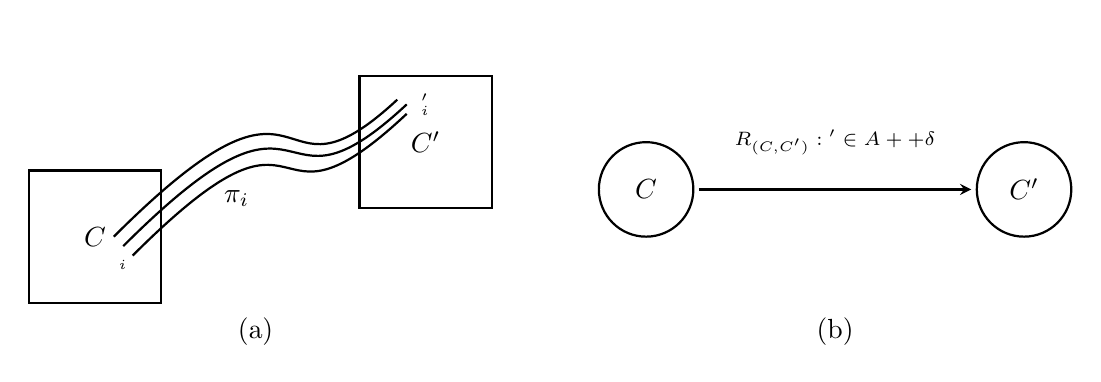
\begin{tikzpicture}
\begin{scope}[scale=1.2]

    \draw [line] (-5.2,-1.2) rectangle (-3.8,0.2);
    \draw [line] (-1.7,-0.2) rectangle (-0.3,1.2);
    \draw [line] (-4.1,-0.7) .. controls +(2.0,2.0) and +(-1.6,-1.5) ..  (-1.2,0.8);
    \draw [line] (-4.2,-0.6) .. controls +(2.1,2.1) and +(-1.5,-1.4) ..  (-1.2,0.9);
    \draw [line] (-4.3,-0.5) .. controls +(2.2,2.2) and +(-1.4,-1.3) ..  (-1.3,0.95);

\node at (-4.5, -0.5) {$C$};
\node at (-1, 0.5) {$C'$};
\node at (-4.2,-0.8) {\scriptsize{$\x_i$}};
\node at (-1.0,0.90) {\scriptsize{$\x_i'$}};
\node at (-3,-0.1) {$\pi_i$};
\node at (-2.8, -1.5) {(a)};
\end{scope}

\begin{scope}[xshift=4.0cm,scale=1.2]
\draw [line] (-2.0,0) circle (0.5);
\draw [line] (2.0,0) circle (0.5);
\draw[arw] (-1.5,0) -- (1.5,0);
\node at (-2.0,0) {$C$};
\node at (2.0,0) {$C'$};
\node at (0,0.5) {\scriptsize{$R_{(C,C')}:\setof{\x' \in A\x + \vb + \delta}$}};
\node at (0.,-1.5) {(b)};
\end{scope}
\end{tikzpicture}
\end{center}
\vspace*{-.3cm}
\caption{(a) Trajectory segments $\traj_i$ are used to compute the
relation $R_{(C,C')}$ that annotates the edge in (b).
$R_{(C,C')}:\setof{\x' \in A\x + \vb + \delta}$ is an interval affine
relation defined by an affine map (matrix $A$ and vector $\vb$) and an
error interval (vector of intervals $\delta$).}
    \label{fig:enriched-edge}
\vspace*{-.3cm}
 \end{figure}


Recall that each edge $(C,C')$ of the graph $G$ denotes an observed
trajectory between the respective cells. The graph abstraction $G$
only states that there exists a state $\x \in C$ from which the system
can evolve to a future state $\x' \in C'$. To increase the precision,
iterative refinement of the abstraction by state splitting was
proposed in~\cite{zutshi2014multiple}. Due to the curse of
dimensionality, state splitting is not scalable. Instead, we propose
an `enrichment' $G^R$ of $G$ by computing a set of local relations
$R_{(C,C')}(\x,\x')$ for every edge $(C,C')$, which
non-deterministically describe relations between $\x \in C$ and $\x'
\in C'$. This is illustrated in \figref{enriched-edge}.
%(compare with \figref{segtraj}).

The enriched graph $G^R$ captures the underlying local forward
dynamics describing the evolution of the system in each abstract
state. We represent the dynamics using an affine model with an
interval error. Such a model can either be approximated using learning
methods or computed as a sound (over) approximation using reachability
set computation methods. Because we assume black box semantics, we
only present the former. Using regression analysis on a witnessed
trajectory between two cells, we compute an approximate discrete map
along with an error estimate.  Moreover, using the simulation function
$\simulate$, additional trajectories (or data) can be generated if
required. The data can be separated into a training set and testing
set to compute the map and the error respectively.

%The latter case can be explored if
%the symbolic dynamics of the system are known. A tool like
%\flowstar~\cite{chen2013flow} can be used to find the reachable set
%map.

Observe that $G^R$, a directed reachability graph, is rich enough to
search for concrete behaviors in the system. We call it a time
parameterized PWA relational abstraction. It can be interpreted as an
infinite state discrete transition system, and we can use
off-the-shelf bounded model checkers to find concrete violations of a
given safety property, and even other temporal properties.

%We now
%discuss the background required to present our ideas.

